%"###############################################
%
% Classification VPPBS post 
%
%###############################################

Pour rechercher le nombre optimal de classes, nous avons évalué, figure~\ref{fig-vppbs-post-elbow} la silhouette moyenne des classes pour un partitionnement de 2 à 20 classes. Il en ressort un pic net (en rouge) à 4 classes, mais la valeur maximale de la silhouette moyenne est atteinte pour k = 12 classes.

\begin{figure}[H]
\centering
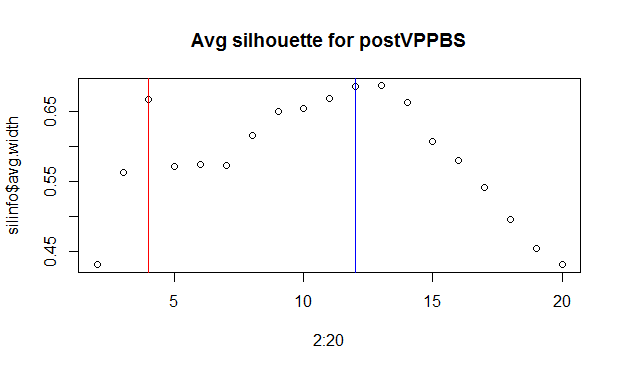
\includegraphics[width=0.75\textwidth]{../Fig/VPPBS/vppbs-elbow-post.png}
\caption{Recherche du meilleur nombre de classes}
\label{fig-vppbs-post-elbow}
\end{figure}

Jetons un bref coup d'oeil sur les silhouettes de classes pour le partitionnement à 4 classes (Cf. figure \ref{fig-vppbs-post-pam-k4}. Nous pouvons y observer 3 classes très solides (valeurs de silhouette entre 0.9 et 1), non triviales (contrairement à certaines classes observées pour les données post-opératoires RTUPB), et chacune de ces classes compte 3 ou quatre patients ; la quatrième classe rassemble tous les autres profils (22 patients sur 32), avec une silhouette de classe assez faible (0.55). Les 3 premières classes observées ici se détachent nettement et nous les retrouverons donc dans le partitionnement à k = 12 classes qui, compte tenu de la silhouette moyenne maximale, devrait faire apparaître de nouvelles classes parmi les 22 profiles restant. Les silhouettes correspondant à ce partitionnement à 12 classes font ressortir, figure~\ref{fig-vppbs-post-pam-k12}:
\begin{itemize}
\item 6 classes de profils fortement corrélés (silhouette > 0.7)
\item seulement 2 classes de profils peu ou pas corrélés (silhouette < 0.5)
\end{itemize}

\begin{figure}[H]
\centering
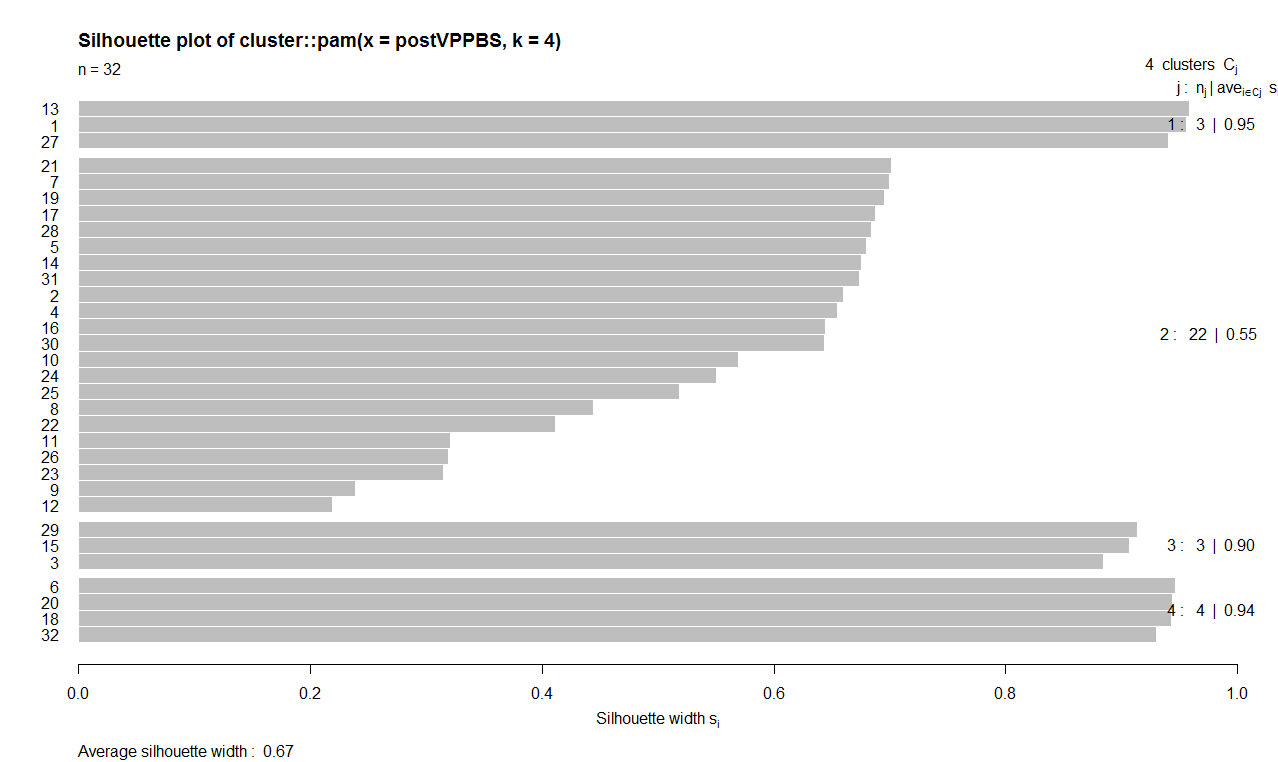
\includegraphics[width=0.75\textwidth]{../Fig/VPPBS/vppbs-sil-k4-post.png}
\caption[]{Silhouette / classe (k = 4)}
\label{fig-vppbs-post-pam-k4}
\end{figure}


\begin{figure}[H]
\centering
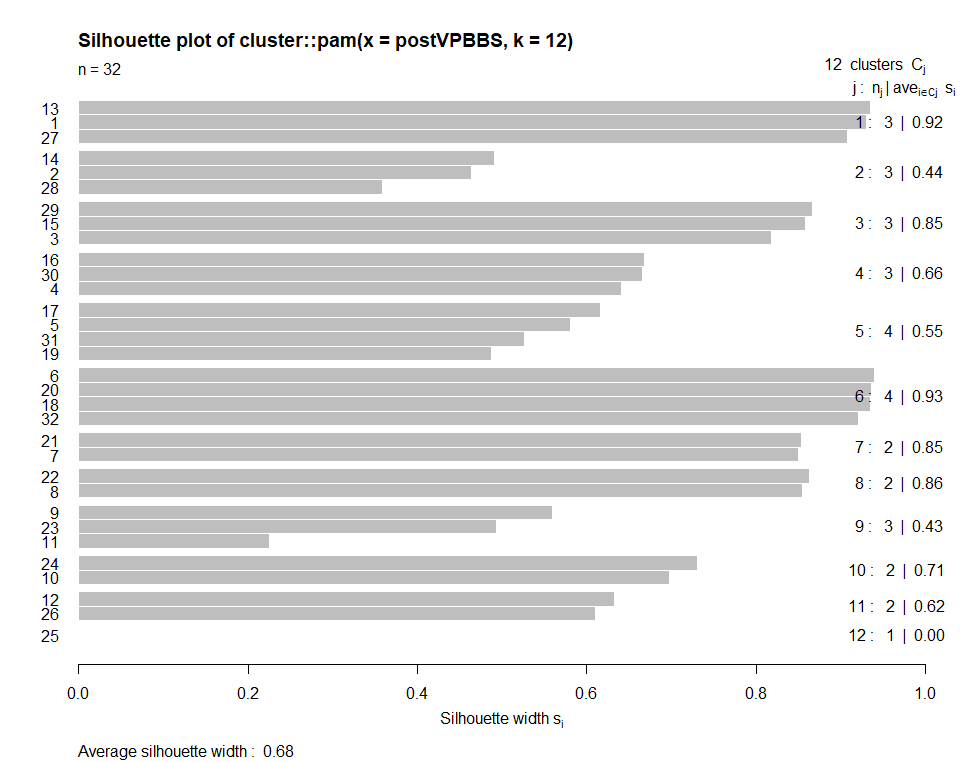
\includegraphics[width=0.75\textwidth]{../Fig/VPPBS/vppbs-sil-k12-post.png}
\caption{Silhouette / classe (k = 12)}
\label{fig-vppbs-post-pam-k12}
\end{figure}

La classification hiérarchique des données post-opératoires VPPBS produit le dendogramme présenté figure~\ref{fig-vppbs-post-cah}. La coupure de l'arbre peut s'effectuer soit à 5 classes (représentées en rouge), soit à 12 classes (représentées en bleu). Le partitionnement à 12 classes correspondant à celui obtenu par la méthode, nous le retiendrons pour étudier les profils post-opératoires. Au besoin, si cela se justifie par la suite, nous factoriserons pour revenir à un partitionnement à 5 classes.

\begin{figure}[H]
\centering
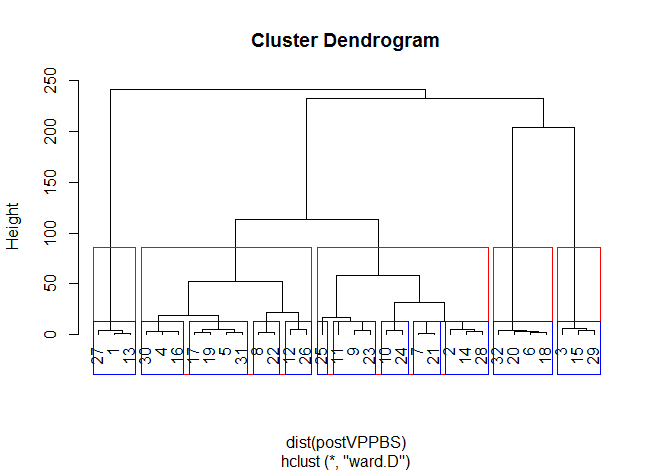
\includegraphics[width=0.75\textwidth]{../Fig/VPPBS/vppbs-cah-k12-post.png}
\caption{VPPBS: Classification hiérarchique}
\label{fig-vppbs-post-cah}
\end{figure}

%
%##########################
%# CONCLUSION
%##########################